\documentclass[../main.tex]{subfiles}
\graphicspath{{\subfix{../img/}}}

\begin{document}

\section{Gating Functions and Parameters for Implemented Models} \label{appendix:functions_and_parameters}

\subsection{Wang 1994}

% \noindent\textbf{T-type Ca$^{2+}$ channel}

% Steady state activation:
% \begin{equation*}
%     s_\infty=\frac{}{}
% \end{equation*}

\textcolor{red}{Sag is commonly referred to as H-current, or corresponding channels - \gls{hcn} channels}

\FloatBarrier

\begin{figure}[!h]
    \centering
    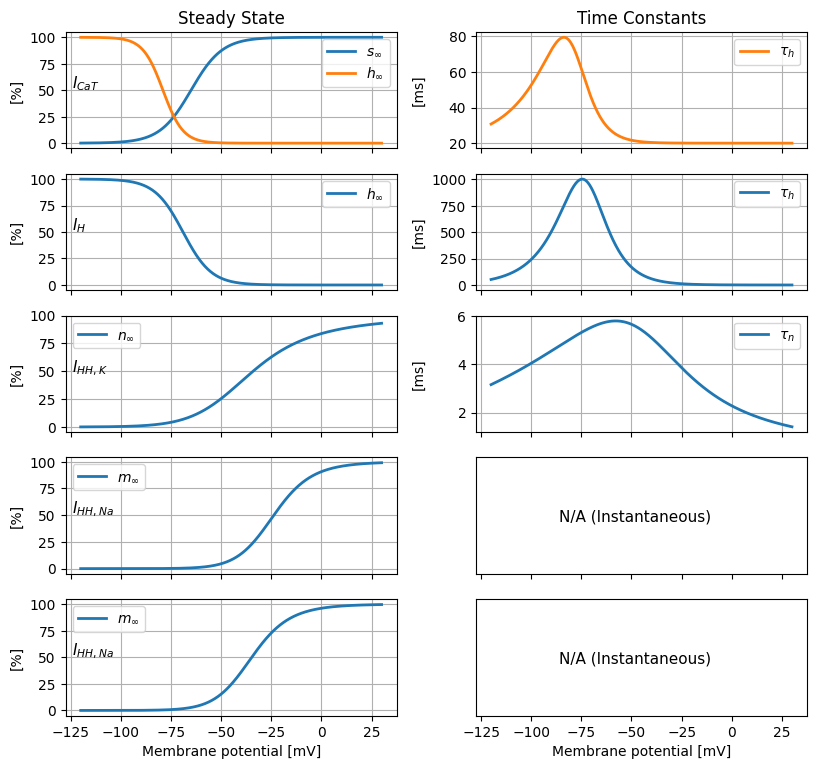
\includegraphics[width=\linewidth]{../img/model_kinetics/kinetics_wang.png}
    \caption[Wang 1994]{
        \textcolor{red}{TODO: Text}
    }
    \label{fig:kinetic_plots_wang1994}
\end{figure}

\FloatBarrier

\textcolor{red}{ToDo}

\subsection{Goldman et. al. 2001}

\textcolor{red}{ToDo}

\subsection{Park et. al. 2021}

\textcolor{red}{ToDo}


%%%%%%%%%%%%%%%%%%%%%%%%%%%%%%%%%%%%%%%%%%%%%%%%%%%%%%%%%%%%%%%%%%%%%%%
\subsection{EAG Channel} \label{appendix:parameters_eag_channel}



\begin{table}[t!]
    \centering
    \begin{tabular}{|l||c|c|c|}
    \hline
    \textbf{Model} & $a$ & $d$ & $k$ \\
    \hline
    \hline
    Default \parencite{bronkRegulationEagCa22018}  & $1$       & $0$        & $16.94$ \\
    Wang 1994     & $0.01$    & $-35.5$    & $0.2$  \\
    Goldman 2001  & $1$       & $0$        & $4$    \\
    \hline
    \end{tabular}
    \caption{Parameter values for EAG channels used in implemented models.}
    \label{tab:eag_parameters}
\end{table}


\end{document}